The main advantage of the FEM over finite differences or spectral methods is the ability to handle oddly shaped domains \parencite{erhunmwun2017review}. This section explores solutions to reaction-diffusion equations on oddly shaped domains that would be hard or even impossible to solve using other approaches.

\subsection{A 2D Maze}

In 2D space, I show this using a domain with a maze-like shape. By defining a triangulation within the space (Figure \ref{fig:tris}), the finite element approach can solve the reaction-diffusion system within this abnormal shape.

\begin{figure}[t]
    \centering
    \caption{Solution to the reaction-diffusion system on a $10 \times 10$ maze-like domain}
    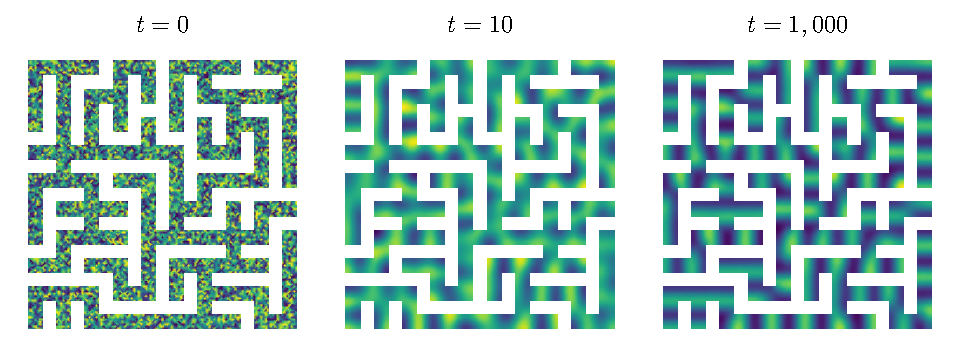
\includegraphics{figures/maze_ts.pdf}
    \label{fig:maze}
\end{figure}

Figure \ref{fig:maze} shows the solution to the PDE with $k_1 = 9$ and $\gamma_v = 0.02$ on this domain. Starting from random noise at $t = 0$, the solution starts to form structure by $t = 10$, and form Turing patterns at $t = 1,000$ in the steady state. Interestingly, the lines within the Turing patterns are all either parallel or perpendicular to the boundary. Because the spacing between lines is relatively consistent, the patterns roughly line up with each other. They do slightly misalign, however, especially on the right side, demonstrating the effect of the domain choice on the solution.


\subsection{3D Surfaces}

Because the surface of 3D shapes can also be triangulated, I can also use the FEM to solve the system along 3D surfaces. My approach ignores the effect of the curvature of the surface, which can affect the shape of the patterns that emerge \parencites{staddon2024zebra}{leon2021full}. Still, it gives a good approximation for the solution of the system on the surface.

\begin{figure}[t]
    \centering
    \caption{Solution to the reaction-diffusion system on 3D surfaces}

    \begin{subfigure}{\textwidth}
        \centering
        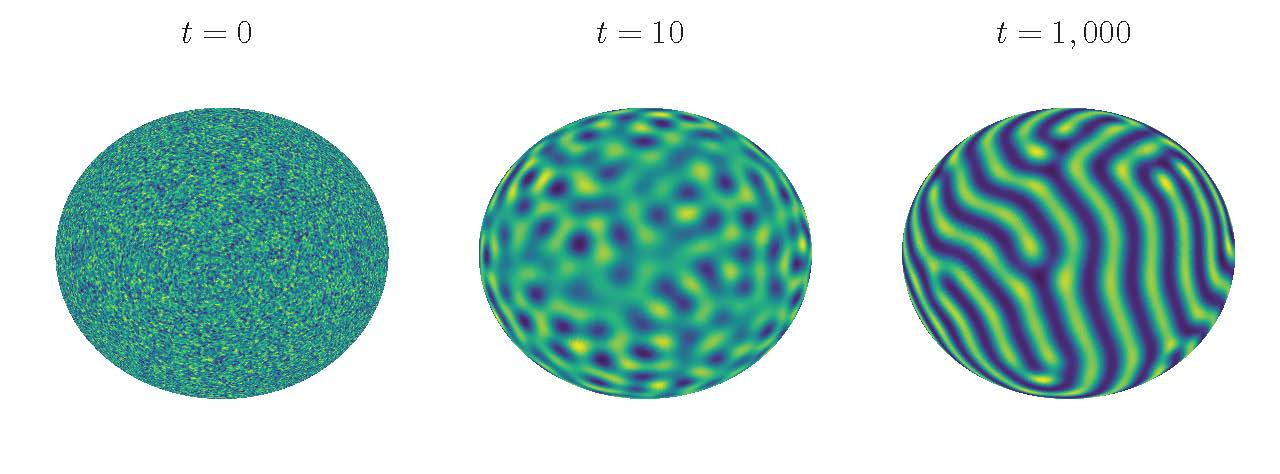
\includegraphics{figures/sphere_ts.pdf}
        \caption{Radius 5 sphere domain}
        \label{subfig:sphere}
    \end{subfigure}

    \begin{subfigure}{\textwidth}
        \centering
        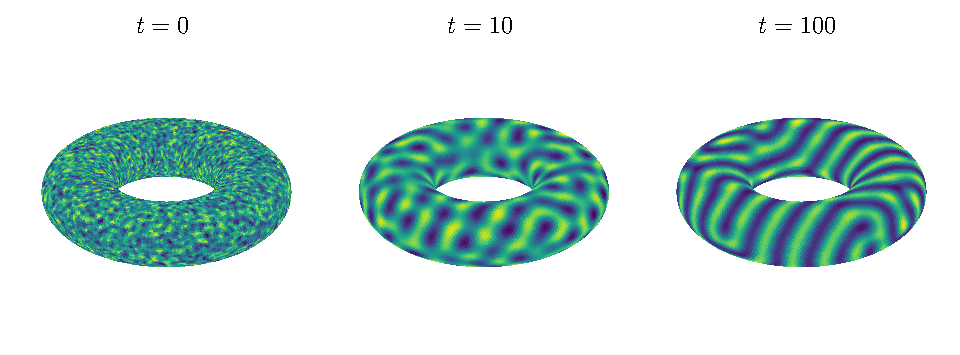
\includegraphics{figures/torus_ts.pdf}
        \caption{$R = 3.5$, $r = 1.5$ torus domain}
        \label{subfig:torus}
    \end{subfigure}

    \label{fig:3d-shapes}
\end{figure}

Figure \ref{fig:3d-shapes} shows the solution to the system with $k_1 = 9$ and $\gamma_v = 0.02$ on two 3D surfaces. Panel \ref{subfig:sphere} shows the solution along a sphere and Panel \ref{subfig:torus} shows the solutions along a torus. Each point in the triangulation for both shapes is connected to its neighbors with no seam, unlike \autocite{leon2021full}, so we allow for diffusion across the whole domain.

The solutions on both surfaces follow the same general pattern as the solution on 2D domains in Figures \ref{fig:sol-ts} and \ref{fig:maze}. At $t = 0$, the domain is covered in random noise. Then, at $t = 10$, we see basic structure emerging before clear Turing patterns appear at $t = 1,000$ in the steady state. On the torus, the lines in the Turing pattern are almost completely parallel to each other while on the sphere more complex patterns develop.
